\documentclass[tikz,border=4pt]{standalone}
\usepackage{tikz}
\usetikzlibrary{calc,arrows.meta,positioning,shapes.geometric}

\begin{document}
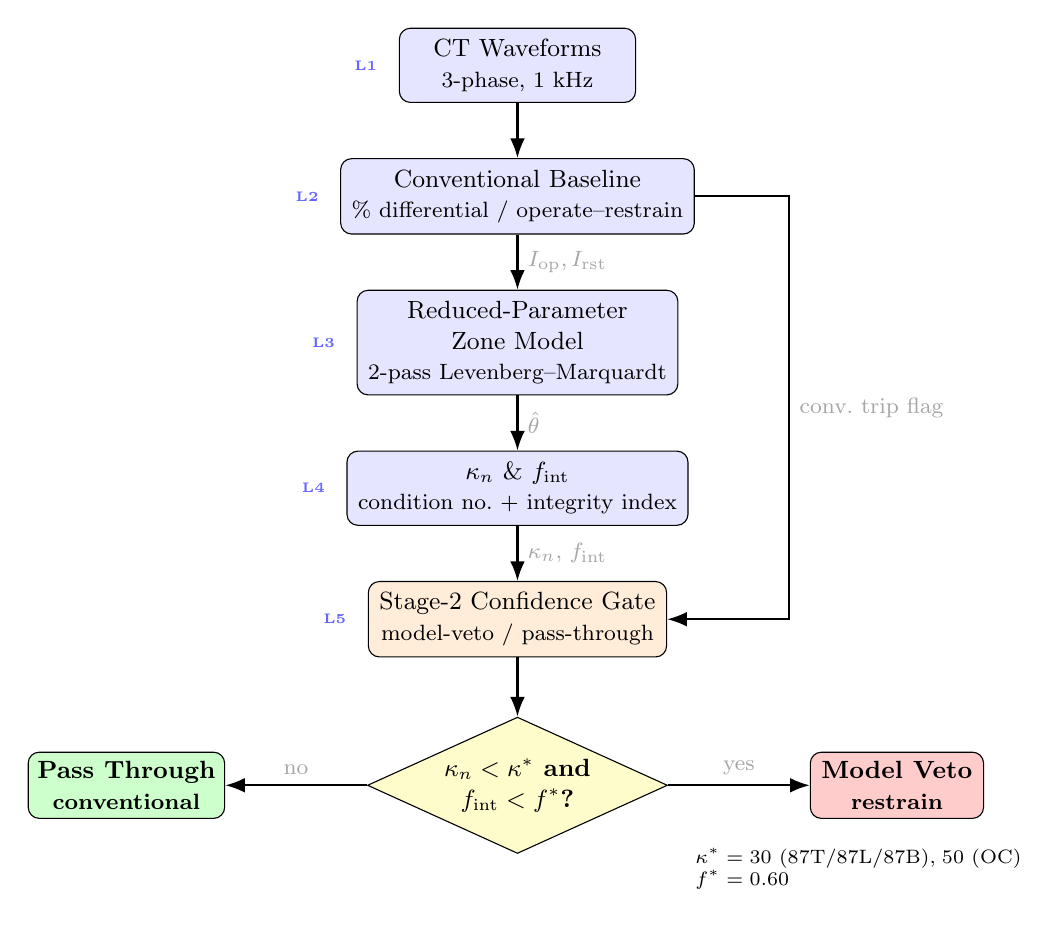
\begin{tikzpicture}[
    block/.style={draw,fill=blue!10,rounded corners=4pt,
                  minimum width=3.0cm,minimum height=0.75cm,
                  font=\small,align=center,inner sep=4pt},
    gate/.style={draw,fill=orange!15,rounded corners=4pt,
                 minimum width=3.0cm,minimum height=0.75cm,
                 font=\small,align=center,inner sep=4pt},
    decision/.style={draw,fill=yellow!20,diamond,aspect=2.2,
                     minimum width=2.8cm,minimum height=0.7cm,
                     font=\small\bfseries,align=center,inner sep=2pt},
    output/.style={draw,fill=green!20,rounded corners=4pt,
                   minimum width=2.2cm,minimum height=0.65cm,
                   font=\small\bfseries,align=center},
    suppress/.style={draw,fill=red!20,rounded corners=4pt,
                     minimum width=2.2cm,minimum height=0.65cm,
                     font=\small\bfseries,align=center},
    arr/.style={-{Latex[length=2.5mm]},line width=0.8pt},
    label/.style={font=\footnotesize,text=gray!70},
]

\def\dx{0}

% ---- Layer 1: CT waveforms -----------------------------------------------
\node[block] (L1) at (0,0) {CT Waveforms\\ \footnotesize 3-phase, 1~kHz};

% ---- Layer 2: Conventional baseline --------------------------------------
\node[block,below=0.7cm of L1] (L2)
    {Conventional Baseline\\ \footnotesize \% differential / operate--restrain};

% ---- Layer 3: Zone model (LM estimator) ----------------------------------
\node[block,below=0.7cm of L2] (L3)
    {Reduced-Parameter\\ Zone Model\\ \footnotesize 2-pass Levenberg--Marquardt};

% ---- Layer 4: Identifiability / integrity metrics -----------------------
\node[block,below=0.7cm of L3] (L4)
    {$\kappa_n$ \& $f_{\rm int}$\\ \footnotesize condition no.\ + integrity index};

% ---- Layer 5: Stage-2 confidence gate -----------------------------------
\node[gate,below=0.7cm of L4] (L5)
    {Stage-2 Confidence Gate\\ \footnotesize model-veto / pass-through};

% ---- Decision diamond ----------------------------------------------------
\node[decision,below=0.75cm of L5] (dec)
    {$\kappa_n < \kappa^*$ and\\ $f_{\rm int} < f^*$?};

% ---- Outputs -------------------------------------------------------------
\node[suppress,right=1.8cm of dec] (veto)
    {Model Veto\\ \footnotesize restrain};
\node[output,left=1.8cm of dec]  (pass)
    {Pass Through\\ \footnotesize conventional};

% ---- Arrows --------------------------------------------------------------
\draw[arr] (L1) -- (L2);
\draw[arr] (L2) -- (L3)
    node[midway,right,label] {$I_{\rm op},I_{\rm rst}$};
\draw[arr] (L3) -- (L4)
    node[midway,right,label] {$\hat\theta$};
\draw[arr] (L4) -- (L5)
    node[midway,right,label] {$\kappa_n,\,f_{\rm int}$};
\draw[arr] (L5) -- (dec);

% Conventional trip feeds gate
\draw[arr] (L2.east) -- ++(1.2,0) |- (L5.east)
    node[near start,right,label] {conv.\ trip flag};

\draw[arr] (dec) -- (veto) node[midway,above,label] {yes};
\draw[arr] (dec) -- (pass) node[midway,above,label] {no};

% ---- Thresholds annotation ----------------------------------------------
\node[font=\scriptsize,align=left,
      below=0.25cm of veto.south east,anchor=north east,xshift=0.6cm]
    {$\kappa^*=30$ (87T/87L/87B),\;50 (OC)\\
     $f^*=0.60$};

% ---- Side label: layer numbers -----------------------------------------
\foreach \n/\y in {1/0, 2/-1.45, 3/-2.9, 4/-4.35, 5/-5.8}
    \node[font=\tiny\bfseries,text=blue!60,left=0.15cm of L\n] {L\n};

\end{tikzpicture}
\end{document}
